
Let 
\begin{align}
	X\in \{0,1,2,3,4,5...\}
\end{align}
We know that, for a poisson random variable $X$ with a given parameter $\lambda$, probability of $X=k$ is:
\begin{align} \label{xe2019-bkup-1:eq_0}
	\pr{X=k}=\left(\frac{\lambda^k e^{-\lambda}}{k!}\right)	
\end{align}
CDF is:
\begin{align}
    F(X=k)=\sum_{x=0}^{k}\left(\frac{\lambda^x e^{-\lambda}}{x!}\right)
\end{align}
   
% The graph of CDF is shown below
% \includegraphics[width=\linewidth]{cdf.png}
And also,
\begin{align}
    \Pr\brak{x < X \le y} = F\brak{y} - F\brak{x}\label{xe2019-bkup-1:eq_1}
\end{align}
Now by using \eqref{xe2019-bkup-1:eq_1},
\begin{align}
    \pr{2 \leq X \leq 4} 
    & = \pr{1 < X \leq 4}\\
    & = F(4)-F(1)\\
    & = \frac{65}{24e}-\frac{2}{e}\\
    & = \frac{17}{24e}
\end{align}
\begin{figure}[ht]
    \centering
    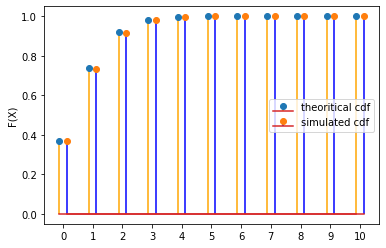
\includegraphics[width=\columnwidth]{solutions/xe/2019/simulated_theoritical.png}
    \caption{Theoretical CDF vs Simulated CDF}
    \label{xe2019-bkup-1:Figure_0}
\end{figure}